\documentclass[french,a4paper,12pt]{report}
\usepackage[utf8]{inputenc}
\usepackage[T1]{fontenc}
\usepackage{graphicx}
\usepackage{float}
\usepackage{listings}
\usepackage{color}
\definecolor{dkgreen}{rgb}{0,0.6,0}
\definecolor{gray}{rgb}{0.5,0.5,0.5}
\definecolor{mauve}{rgb}{0.58,0,0.82}

\lstset{frame=tb,
  language=Java,
  aboveskip=3mm,
  belowskip=3mm,
  showstringspaces=false,
  columns=flexible,
  basicstyle={\small\ttfamily},
  numbers=none,
  numberstyle=\tiny\color{gray},
  keywordstyle=\color{blue},
  commentstyle=\color{dkgreen},
  stringstyle=\color{mauve},
  breaklines=true,
  breakatwhitespace=true,
  tabsize=3
}


\title{LO52\\ Travaux Pratiques 1 :\\ Introduction à l'AOSP}
\author{Professeur encadrant : BRISSET Fabien \\ Elèves : \\ROMET Pierre
\\PROST Guillaume \\ \\ \\}
\date{Automne 2017}

\begin{document}

\maketitle
\tableofcontents

\chapter{Introduction}
Lors de ce premiers tp, nous avons commencé à nous approprier l'univers Android.
Tout d'abord nous avons pris place au sein de l'AOSP mise à notre disposition
en créant une branche: "Tauntaun".

Par la suite, nous avons installé et parametré l'IDE "Android Studio" afin de
pouvoir développer notre première application Android basique, afin de
comprendre les mécanismes propres à l'IDE.

Pour finir, nous avons pris connaissance de notre sujet de tp/projet sur
lequel nous allons être amené à travailler durant le semestre.
Ainsi, nous avons conçu une base de données SQLITE, suivant le model UML
"ER DIAGRAM", devant nous permettre de "lister les volants officiels
réglementaires et leurs tarifs afin de gérer leurs stocks au sein des clubs".
De plus, nous avons également commencé l'intégration de la base de données au
sein de notre application.


\chapter{Installation d'Android Studio et Première application}
\section{myFirstApp}
Une fois notre IDE "Android Studio" installé et fonctionnel, nous avons pu
commencer le développement de notre prermière application Android, en suivant
le tutoriel fournie par Google à l'adresse suivante:
"https ://developer.android.com/training/basics/firstapp/index.html"
\subsection{Create an Android Project}
Dans un premier temps, nous avons commencé par la création et le paramétrage
d'un nouveau projet Android en spécifiant les informations suivantes:
\begin{itemize}
  \item Utilisation du SDK lié à Android6.0, nommé "Marshmallow"
  \item L'utilisation d'un projet vide "Empty Activity"
\end{itemize}

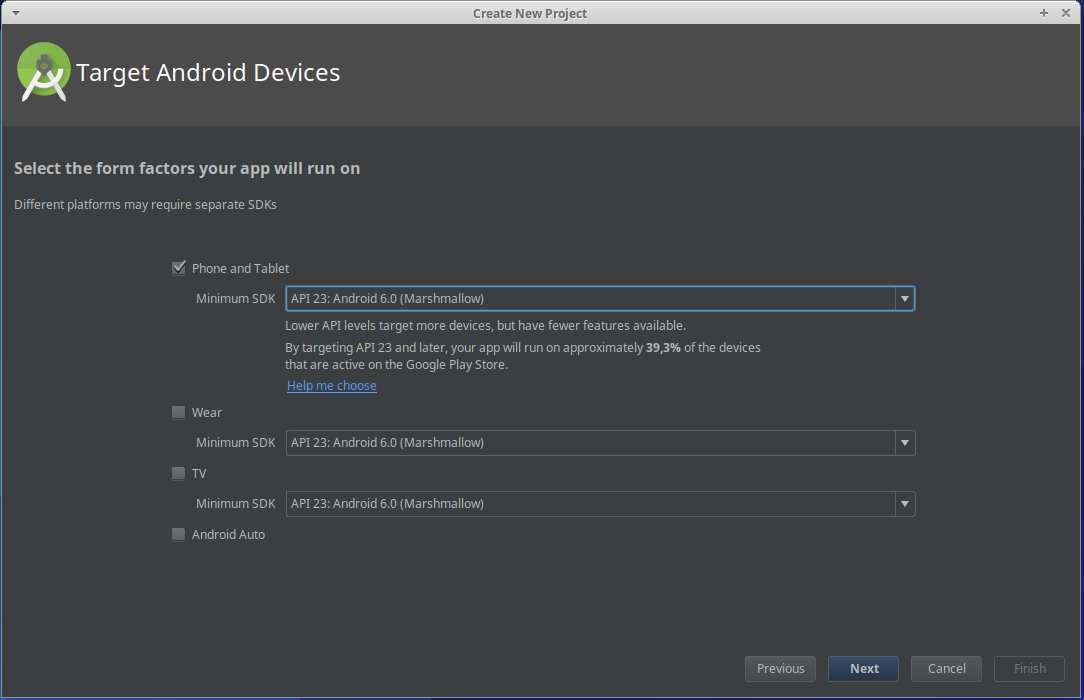
\includegraphics[width=10cm]{3Sdk.png}

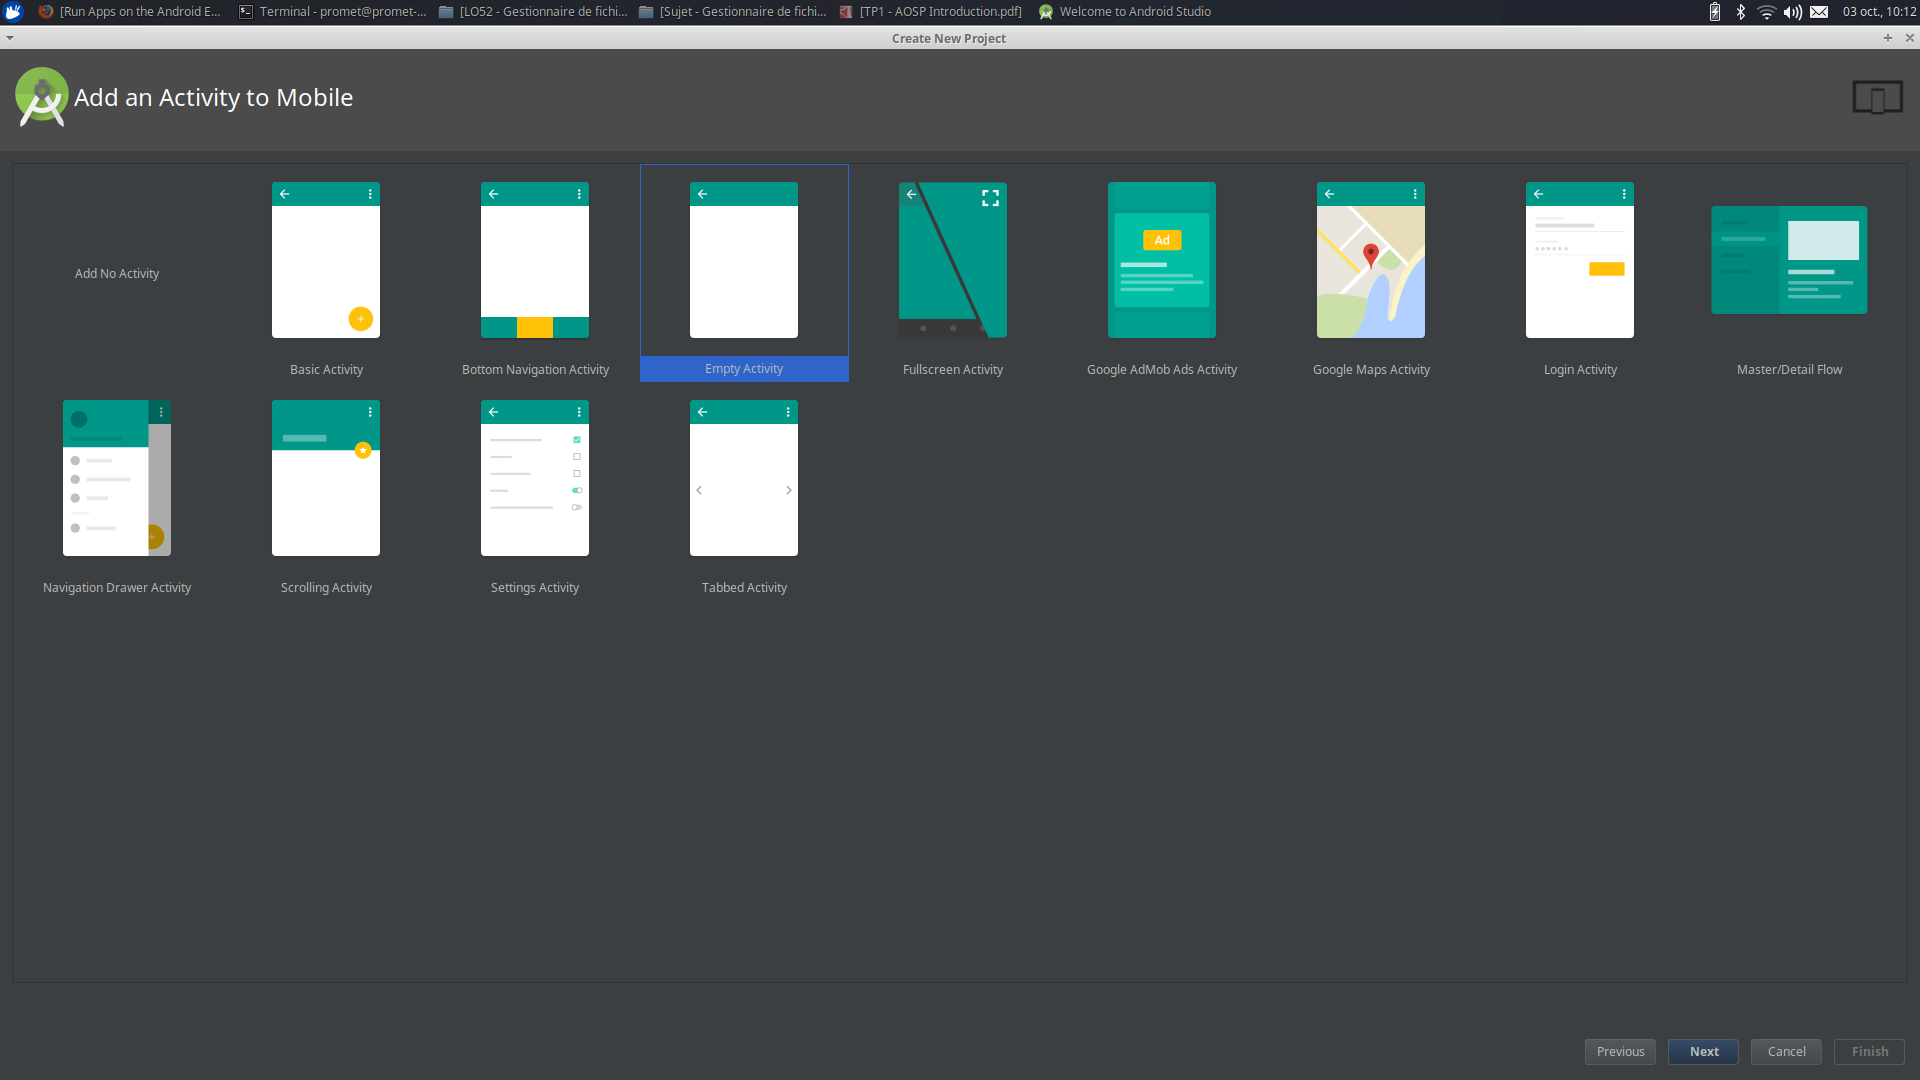
\includegraphics[width=10cm]{4Activity.png}

\subsection{Run our Android aplication}
Par la suite, nous avons cherché à déployer notre application sur une cible.
Pour cela, deux moyens s'offre à nous au sein d'Android Studio, nous pouvons
déployer notre application au choix, sur un smartphone, en connectant celui-ci
à notre station de travail, ou au sein de l'émulateur mise à disposition par
notre IDE.

Dans le cas du déploiement sur smartphone, il est nécessaire de disposer des
driver de ce dernier, afin d'assurer reconnaissance de l'appareil par notre
IDE.De plus, il est également nécessaire d'activer "l'USB debugging" sur le
téléphone, via le menu "Developper options".

Dans le cas d'un déploiement sur émulateur, il est nécessaire de configurer ce
dernier, comme illustré ci-dessous.

On lance " Android Virtual Device Manager" en sélectionnant "Tools > Android > AVD Manager",
puis l'on peut créer un nouvel "virtual device", en cliquant sur "Create Virtual Device".

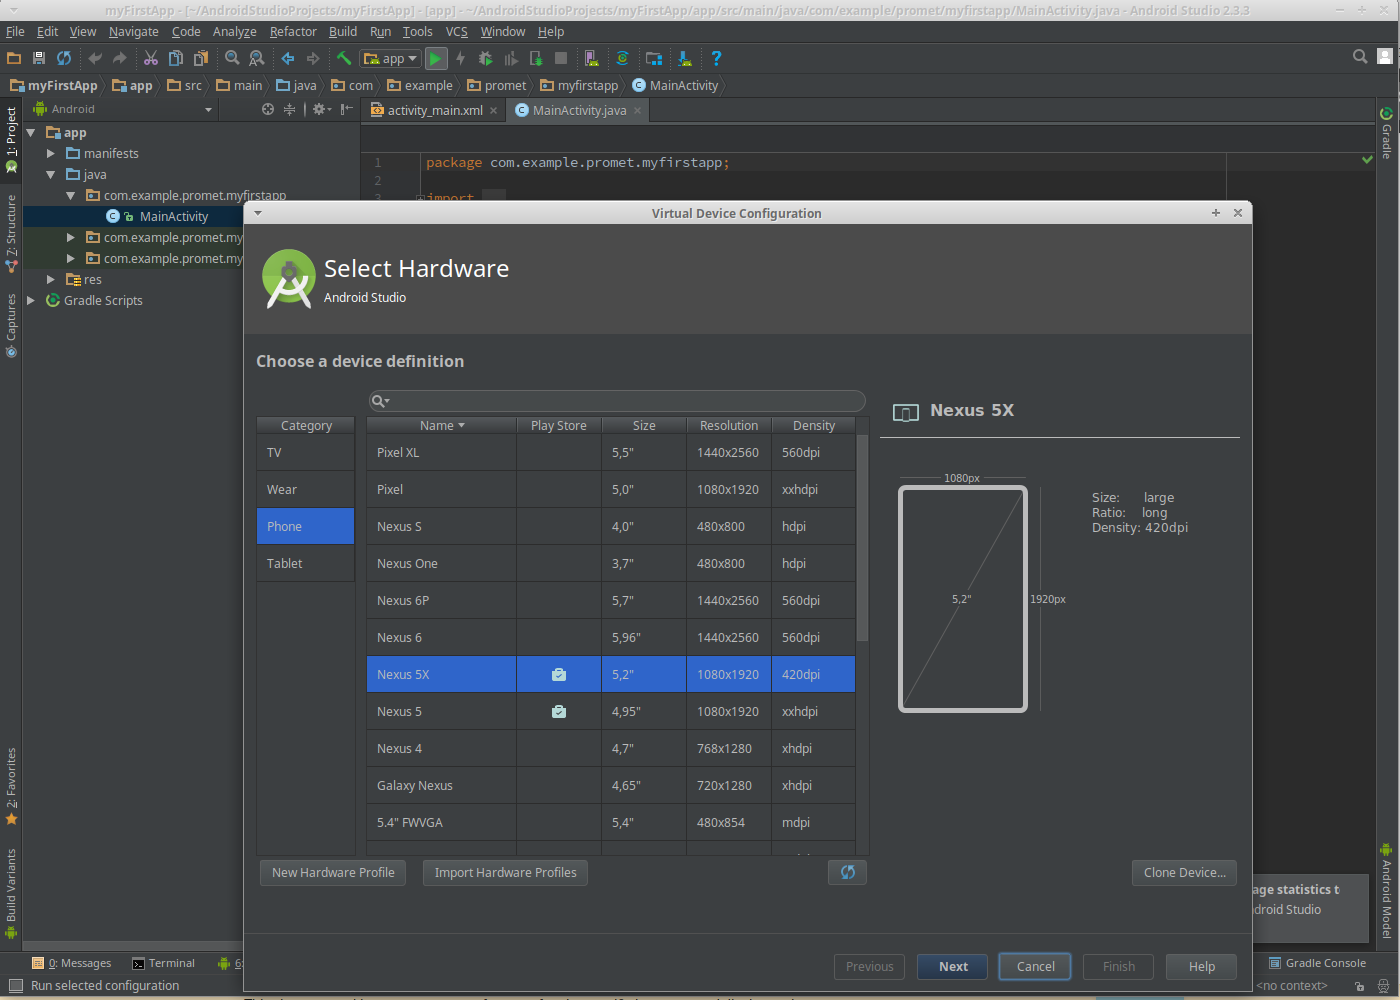
\includegraphics[width=9cm]{7.png}

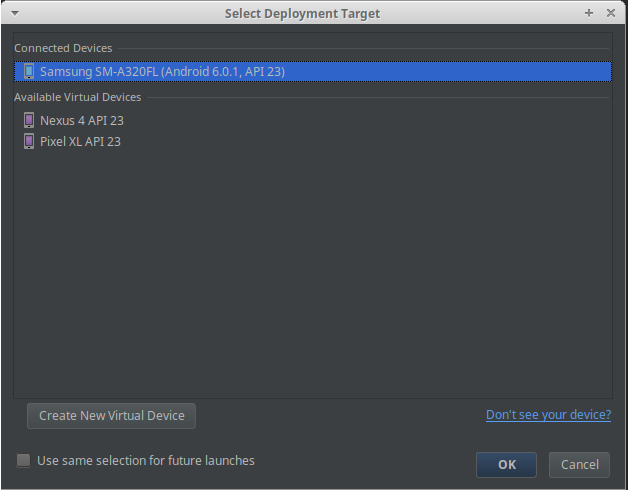
\includegraphics[width=9cm]{121.png}

\subsection{Build a Simple User Interface}

Enfin nous avons vu comment, grâce à l'utilisation des "Layouts" et des "widgets",
mettre en place une interface graphique (UI) basique, mettant en jeux, des éléments
"plainText" ainsi que des éléments "buttons".
\bigbreak
L'interface graphique sous Android utilise une hiérarchie de layouts (ViewGroup object)
ainsi que de widget(View objects).
\smallbreak
Le Layout traduit un conteneur invisible, qui permet le positinnement des éléments
qu'il contient ("child view") sur l'écran.s
\smallbreak
Les widgets, quant à eux, sont des composants graphiques tel que des buttons ou
encore des textBoxes.

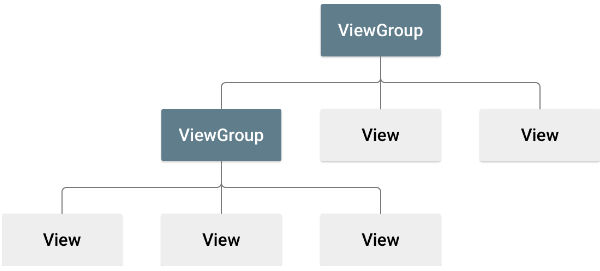
\includegraphics[width=10cm]{13.png}

\subsection{Open the Layout Editor}
L'objectif de cette partie était de nous permettre de prendre en main, les
différents mode d'ancrage (ainsi que les paramètres qui lui sont lié "Default
Margins") d'un éléménts tel qu'une "textBoxe". A travers l'affichage "Show
Blueprint" nous avons pu, graphiquement, effectuer ces actions.

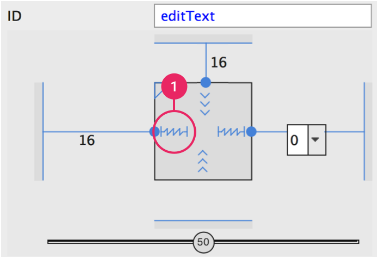
\includegraphics[width=10cm]{131.png}

\subsection{Text box && a button}
Par la suite, nous avons ajouté une textBoxe ainsi qu'un bouton afin de pouvoir
commencer à intéragir avec notre applications.

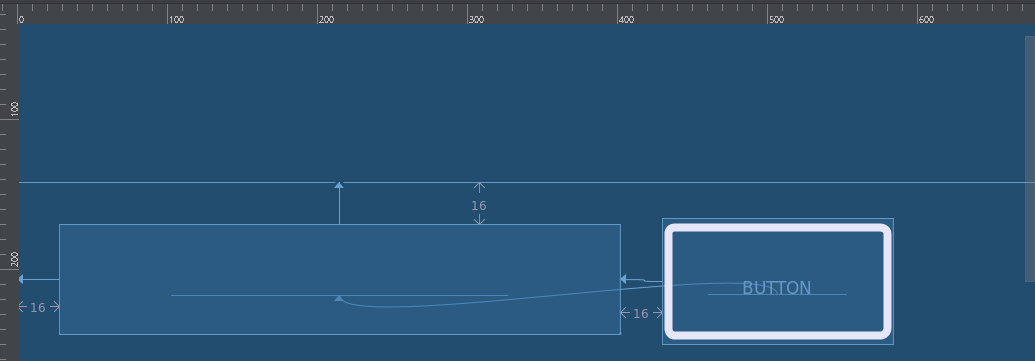
\includegraphics[width=10cm]{15.png}

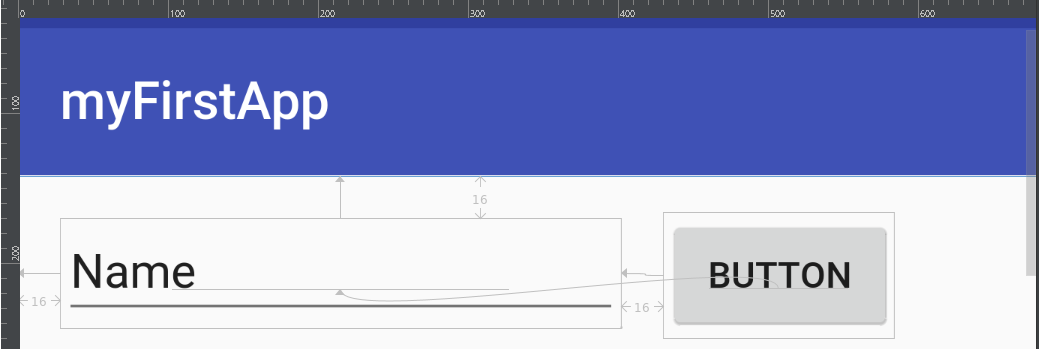
\includegraphics[width=10cm]{16.png}
\bigbreak
Maintenant que nos éléments sont placés, il serait intéressant de pouvoir modifier
le texte (String) qu'il affiche par défaut. Pour cela, Android met en place un
fichier "strings.xml", qui contient toutes les Strings utilisés au sein de notre
interface graphique. Nous allons donc ajouter deux éléments String à ce fichier,
que nous lierons par la suite à nos éléments.
\smallbreak
Nous utilisont donc l'outil "translate editor", fournissant une UI afin d'ajouter
nos éléments au fichier.
\bigbreak
pour finir, nous avons du lier notre fichier conteneurs de String avec nos
éléments graphique, afin que l'affichage s'adapte de manière automatique.
\bigbreak
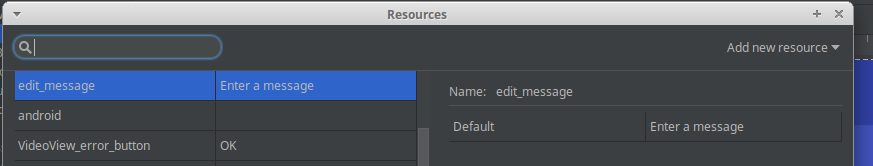
\includegraphics[width=10cm]{19.png}

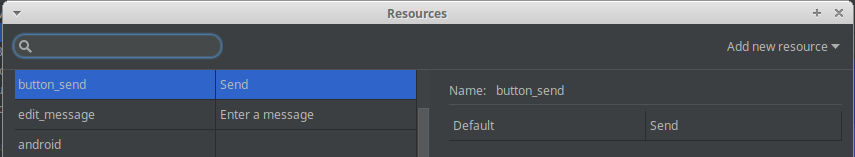
\includegraphics[width=10cm]{20.png}

\subsection{Responsive size}
Afin que notre application puisse s'adapter à différente taille d'écran, il est
nécessaire de mettre en place un affiche dit "responsive" qui à la particularité
de s'adapter automatiquement aux différentes tailles d'écran possible.

Nous avons ainsi du modifier les paramètres d'ancrage, spécifiant l'utilisation
de "match constraints", afin de bénéficier d'un positionnement dynamique.

\section{Start another activity}
Après avoir mis en place l'activité précédente, nous pouvons maintenant utiliser
des éléments permettant une interaction avec notre application. Nous allons voir
au sein de cette partie, comment lier le déclanchement d'une nouvelle "activity" avec
l'appui sur un élément "button".
\bigbreak
Nous avons tout d'abord du créer une méthode déclanché par un appui sur un
élément "button".
\bigbreak
 Ensuite, au sein de notre activité principal, nous avons mise en place un "intent",
 qui est un élément permettant de relier deux éléments graphiques distinct, tel
 que deux "activity". Dans notre cas, cet "intent" nous permettra de déclancher
 le lancement de la deuxième "activity".
 \bigbreak

 \begin{figure}[h]
     \begin{minipage}[c]{.46\linewidth}
         \centering
         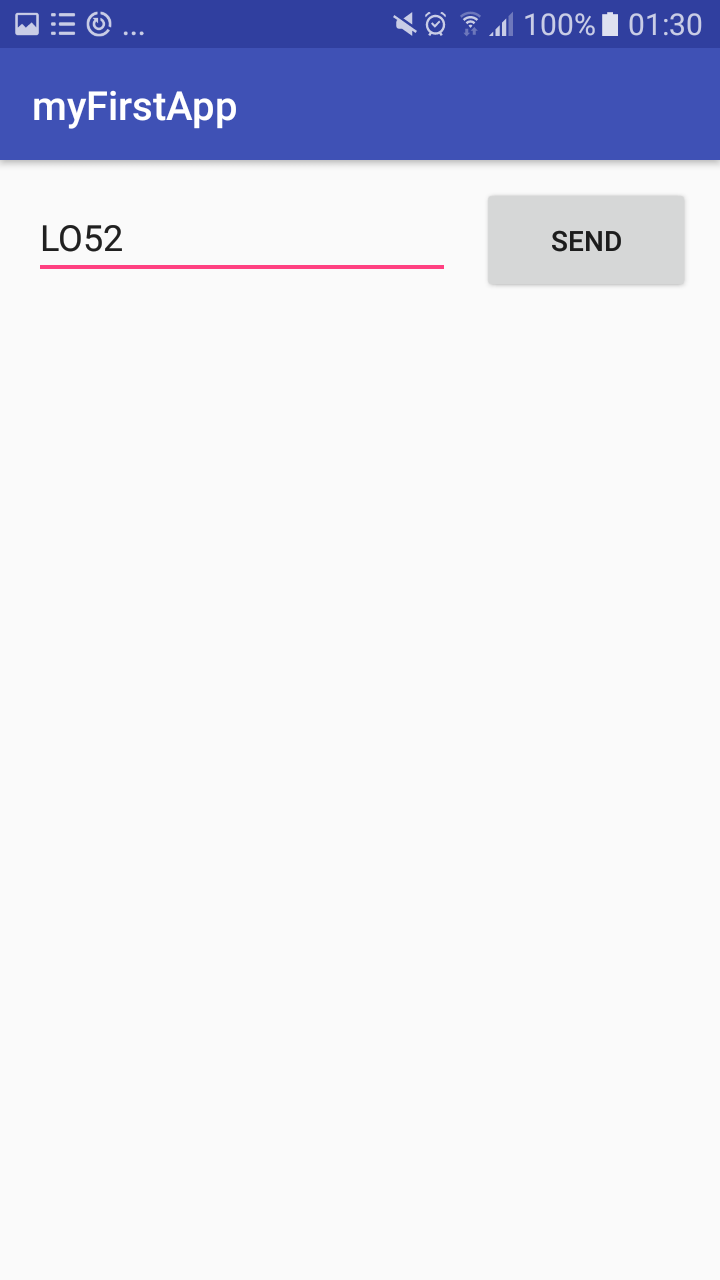
\includegraphics[width=5cm]{21.png}
     \end{minipage}
     \hfill%
     \begin{minipage}[c]{.46\linewidth}
         \centering
         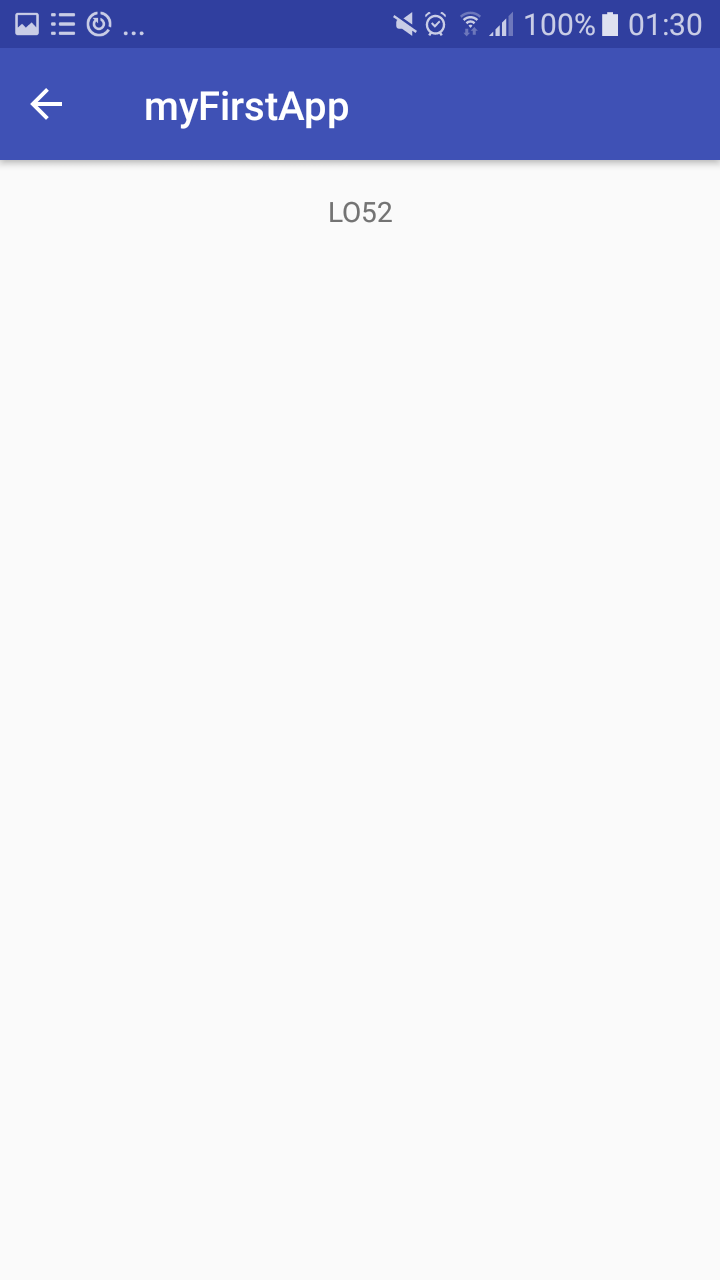
\includegraphics[width=5cm]{22.png}
     \end{minipage}
 \end{figure}

\bigbreak
Pour finir, comme nous pouvons le voir sur le document ci-dessus, nous pouvons
afficher un message envoyé par la première "activity" au sein de la seconde.
De plus, nous avons ajouté un bouton de navigation afin de pouvoir évoluer
entre nos deux "activity".

\chapter{Base de données, modélisation et intégration}
Pour concevoir l'architecture des tables que nous utiliserons pour notre base
de données, nous avons décidé de commencer par représenter un volant et ses
différentes données en dehors de l'aspect commercial (prix, stock, etc...),
et d'ensuite nous attarder sur ce dernier.

\section{Le volant et son constructeur}
Pour la FFBAD, un volant est un produit composé d'une référence et d'une marque
auquel sont associés diverses données permettant de le classifier, tel qu'une
note fédérale déterminant dans une certaine mesure sa qualité. Cette note est déterminé
par un rapport d'analyse réalisé par un laboratoire. De plus, un volant est
éligible pour une saison donnée( ex : saison 2017-2018).

La marque du volant ne correspond pas forcément au nom de l'entreprise l'ayant
produite, ces données doivent donc être séparées. L'entreprise est définie par
son nom, son adresse et son contact, ce dernier étant la personne à contacter
en cas de besoin. Les coordonnées de cette dernière doivent donc également être
 enregistrées.

La représentation de tous ces éléments sous forme de tables se fait donc comme
ceci :

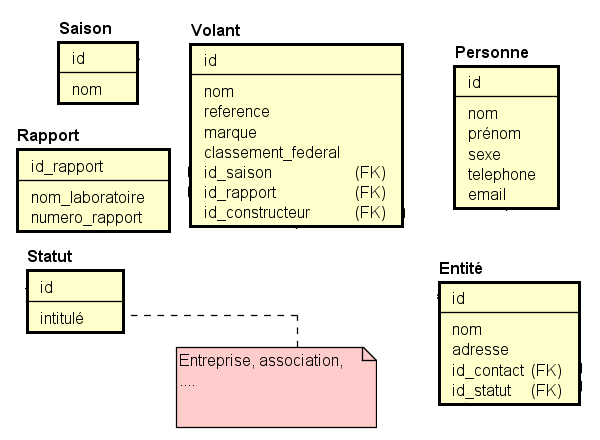
\includegraphics[width=15cm]{ensemble1.png}

Les tables Saison, Rapport et Entité ont été ajouté pour éviter la redondance
d'information : en effet, comme plusieurs volants peuvent avoir les mêmes
valeurs, il est préférable d'utiliser des tables supplémentaires et d'y faire
référence dans la table Volant. Cette dernière possède donc une clé étrangère
vers la saison pour laquelle le volant est éligible, une autre vers le rapport
d'évaluation du volant, et une troisième vers l'entreprise l'ayant fabriqué.

La table répertoriant les constructeurs a été nommée Entité car elle ne stocke
pas que des constructeurs, mais contient également d'autres entreprises (pas
forcément des constructeurs) ainsi que des associations et des particuliers.
Cette table contient donc des champs génériques (nom, adresse), et référence un
 statut ainsi qu'un contact. Nous avons déjà parlé du principe du contact
 précédemment, mais le statut est une donnée nouvelle que nous avons rajouté
 suite à notre choix d'utiliser la table Entité pour contenir toutes sortes
 d'acteurs/entreprises : ce champ permet de typer nos entités (ndla : des
 exemples de valeur pour ce champ sont indiqués dans le rectangle rose associé
 à la table Entité), et donc d'ajouter un peu de précision relatives aux entités.

Nous avons choisi d'utiliser des relations non-identifiantes entre toutes ces
tables car nous estimons que les clés étrangères présentes dans les tables ne
font partie de l'identité des données des tables dans lesquelles elles sont
présentes (ex : l'identifiant du rapport d'évaluation d'un volant n'est pas
une clé pour identifier un volant parmis d'autre).

\section{commandes de volants}
Passons mainenant à la partie commerciale des données.

Le sujet du TP1 spécifie que du point de vue de la vente, un volant est associé
à un vendeur, et que ce dernier possède un certain nombre de tubes de volant et
fixe lui-même le prix de vente unitaire.

Nous avons donc ajouté une table Produit (voir ci-dessous), possédant deux clés
primaires étrangères : un identifiant de volant et un identifiant de
distributeur, ce dernier étant stocké dans la table Entité. Le choix des deux
clés étrangères en tant que clés primaires est justifié car :
\begin{itemize}
  \item Un distributeur ne peut avoir qu'une seule foit un volant donné dans
  son catalogue.
  \item Un distributeur peut vendre plusieurs volants.
  \item Un volant peut être vendu par plusieurs distributeurs en même-temps.
\end{itemize}
Ces trois points nous indiquent que, dans la table Produit, il ne peut y avoir
au maximum qu'une seule fois une combinaison volant-distributeur donnée, quels
que soient le prix et le stock.

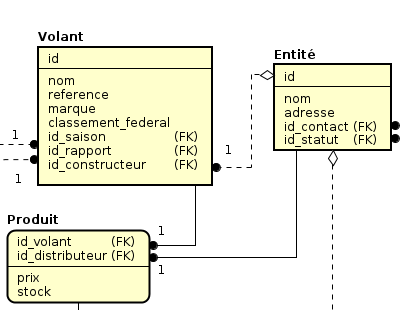
\includegraphics[width=10cm]{ensemble2.png}

Une fois la table Produit ajoutée à l'architecture, il ne reste plus qu'à
ajouter la notion de commandes de produits.

Nous avons pensé ce concept de la manière suivante : une commande de produit
est composé de plusieurs produits, auxquels sont associés le montant désiré.
La commande en elle-même est associé à un acheteur et possède un état binaire :
payé ou non-payée.

Nous avons donc créé une première table Commande définie par un identifiant,
l'état binaire décrit ci-dessus et qui possède une référence vers l'acheteur
(FK de la table Entité).

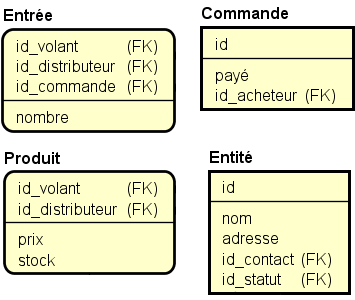
\includegraphics[width=12cm]{ensemble3.png}

Ensuite, nous avons ajouté une seconde table, nommée Entrée, qui correspond à
une ligne de la commande. C'est cette table qui va associer un produit à la
commande, et donc à l'acheteur. L'utilisation de cette seconde table nous permet
 d'avoir des commandes de taille variable et non-limitée.
Chaque entrée est donc définie par un numéro de commande et par un produit.
De cette manière il est, par conception, impossible d'avoir deux entrées ayant
 le même produit dans une commande donnée.
(ndla : nous considérons cela comme un doublon indésirable, puisque la table
Entrée possède un champ destiné à représenter le nombre de tubes de volants désirés)
Une fois ces deux tables ajoutées à notre structure de base de données, nous
obtenons notre structure version 1.0.

\section{Initialisation et connection de la bdd au démarrage de l'appli}
Dans cette toute dernière partie, il nous fut proposé d'essayer d'intégrer notre
base de donnée au sein de l'application que nous venions de créer.

Il nous fallais donc implémenter notre bdd à travers l'outil "SQL Helper", mais
cela impliquait de coder entièrement la modélisation (ER Diagram) que nous
venions de réaliser sous le logiciel "Astah".
Ainsi, décision fut prise de générer un fichier SQLite basé sur notre modélisation,
afin de l'intégrer au sein de notre application. Pour cela, nous avons procéder
comme suivant:

Tout dabord, il a fallu intégrer notre fichier ".SQL" au sein de notre projet.
Pour ce faire, nous insérer dans le dossier "assets", un container spécialisé.
Ensuite, nous avons créer une classe "DataBaseHelper", constitué des méthodes
suivantes:
\begin{itemize}
  \item "createDataBase", permettant de créer une bdd vide, afin de la remplir avec
  nos données.
  \item "checkDataBase", permettant de vérifier si une bdd est déja existante, afin
  d'éviter une recopie à chaque ouverture de l'application.
  \item "copyDataBase", qui nous permet de copier les données de notre fichier ".SQL"
  dans la dbb de l'application.
  \item "openDataBase", permettant d'ouvrir notre base de données.
\end{itemize}
Ainsi, lors de l'ouverture de notre application, nous ne reste plus cas effectuer
un appel à la fonction de création de la bdd, puis de demander son ouverture. \newline

PS:Vous trouverez le code de la classe "DataBaseHelper" en annexe.

\chapter{Annexe}

\begin{lstlisting}
public class DataBaseHelper extends SQLiteOpenHelper
{
    private static String DB_PATH = "/data/data/com.example.promet.myfirstapp/databases/";
    private static String DB_NAME = "Diagrammes_projet_badminton";
    private SQLiteDatabase myDataBase;
    private final Context myContext;

    //Constructor
    public DataBaseHelper(Context context){
        super(context, DB_NAME, null, 1);
        this.myContext = context;
    }

    //Creates an empty database and rewrites it with our own database.
    public void createDataBase() throws IOException{
        boolean dbExist = checkDataBase();
        if(!dbExist){
            //Empty database will be created into the default system path & gonna be able to overwrite that database with our database.
            this.getReadableDatabase();
            try{
                copyDataBase();
            }
            catch (IOException e){
                throw new Error("Error copying database");
            }
        }
    }

    //Check if the database already exist to avoid re-copying each time we open the app
    private boolean checkDataBase(){
        SQLiteDatabase checkDB = null;
        try{
            String myPath = DB_PATH + DB_NAME;
            checkDB = SQLiteDatabase.openDatabase(myPath, null, SQLiteDatabase.OPEN_READONLY);
        }
        catch(SQLiteException e)
        {//database does't exist yet.}

        if(checkDB != null){
            checkDB.close();
        }
        return checkDB != null ? true : false;
    }

     /*Copies your database from your local assets-folder to create empty database
     * This is done by transfering bytestream.*/
    private void copyDataBase() throws IOException{
        //Open your local db as the input stream
        InputStream myInput = myContext.getAssets().open(DB_NAME);

        //Path to the just created empty db
        String outFileName = DB_PATH + DB_NAME;

        //Open the empty db as the output stream
        OutputStream myOutput = new FileOutputStream(outFileName);

        //transfer bytes from the inputfile to the outputfile
        byte[] buffer = new byte[1024];
        int length;
        while ((length = myInput.read(buffer))>0){
            myOutput.write(buffer, 0, length);
        }
        //Close the streams
        myOutput.flush();
        myOutput.close();
        myInput.close();
    }

    public void openDataBase() throws SQLException{
        //Open the database
        String myPath = DB_PATH + DB_NAME;
        myDataBase = SQLiteDatabase.openDatabase(myPath, null, SQLiteDatabase.OPEN_READONLY);
    }
\end{lstlisting}
\end{document}
